\documentclass{beamer}

\mode<presentation> {
\usetheme[secheader]{Madrid}
\usecolortheme{seahorse}
\useinnertheme{circles}
}

\usepackage{graphicx} % Allows including images
\usepackage{booktabs} % Allows the use of \toprule, \midrule and \bottomrule in tables
\usepackage{tikz}
\usepackage{caption}
\usepackage{hyperref}



%----------------------------------------------------------------------------------------
%	TITLE PAGE
%----------------------------------------------------------------------------------------



\title[Hypothesis Testing]{Hypothesis Testing} % The short title appears at the bottom of every slide, the full title is only on the title page

\author{Chaklam Silpasuwanchai} % Your name
\institute[AIT] % Your institution as it will appear on the bottom of every slide, may be shorthand to save space
{
Asian Institute of Technology \\ % Your institution for the title page
\medskip
\textit{chaklam@ait.asia} % Your email address
}
\date{} % Date, can be changed to a custom date

\AtBeginSection[]
{
\begin{frame}<beamer> 
\tableofcontents[currentsection]  % show TOC and highlight current section
\end{frame}
}

\begin{document}

\begin{frame}
\titlepage % Print the title page as the first slide
\end{frame}

\begin{frame}
\frametitle{Overview} % Table of contents slide, comment this block out to remove it
\tableofcontents
 % Throughout your presentation, if you choose to use \section{} and \subsection{} commands, these will automatically be printed on this slide as an overview of your presentation
\end{frame}

%----------------------------------------------------------------------------------------
%	PRESENTATION SLIDES
%----------------------------------------------------------------------------------------

\begin{frame}
\frametitle{Sources} 
\begin{itemize}
	\item Mackenzie, Chapter 6, \textbf{Hypothesis Testing},  Human Computer Interaction: An Empirical Research Perspective, 1st ed. (2013) 
	\item Yatani, Advanced Topics in Human-Computer Interaction, \url{http://yatani.jp/teaching/doku.php?id=2016hci:start}
\end{itemize}
\end{frame}

%\begin{frame}
%	\frametitle{Reminders}
%	\begin{itemize}
%		\item Next week project proposal presentation.  Hard copy and soft copy as usual.
%		\item Next next week, please bring your pc, and install JASP.  We shall together do "Analysis of Variance" workshops for two weeks.
%	\end{itemize}
%\end{frame}


%------------------------------------------------
\section{Analysis of variance} % Sections can be created in order to organize your presentation into discrete blocks, all sections and subsections are automatically printed in the table of contents as an overview of the talk
%-----------------------------------------------

%\begin{frame}
%	\frametitle{Statistical Procedures} 
%	\begin{itemize}
%		\item Statistical tests comes in two forms: \textbf{parametric} and \textbf{non-parametric test}
%		\item Parametric tests operate on data based on assumptions of a normal distribution or the t-distribution.
%		\item Non-parametric tests can operate on any data.
%		\item Parametric tests are superior to non-parametric tests, but require assumptions of distributions.
%	\end{itemize}
%	\begin{figure}
%	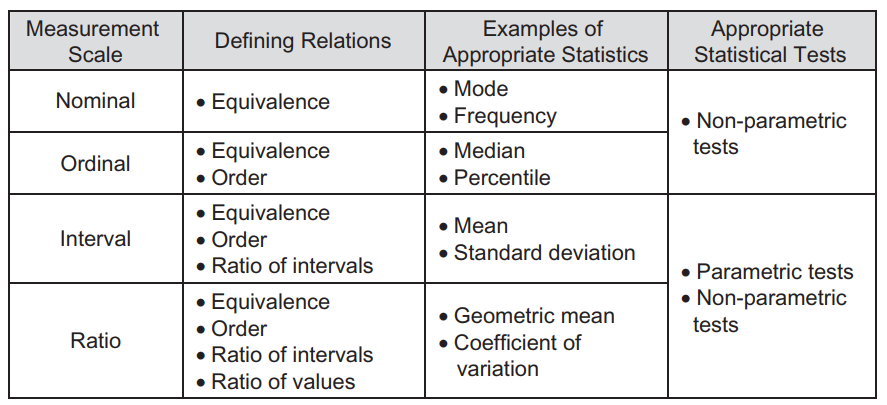
\includegraphics[width=0.6\linewidth]{stat}
%	\caption{Source: Fg. 6.1 (Mackenzie): Measurement scales of data, properties of data, and appropriate statistical tests}
%\end{figure}
%\end{frame}
%
%\begin{frame}
%	\frametitle{Type of data} 
%	\begin{itemize}
%		\item Nominal: techniques, gender, occupation
%		\item Ordinal: likert-scale question; each interval is not equal
%		\item Interval: tmperature; no exact zero
%		\item Ratio: height/weight, speed, accuracy, time
%	\end{itemize}
%\end{frame}
%
\begin{frame}
	\frametitle{Analysis of Variance} 
	\begin{itemize}
		\item \textbf{ANOVA}, or \textbf{F-test}, is the main statistical test for factorial experiment
		\item \textbf{\textit{T} test} is similar but only two levels
		\item The main motivation to use statistical test is - to check that the difference in mean \textbf{occur by chance} or is \textbf{significant}?
%		\item The way to achieve is to determine whether IV has a significant effect on IV is based on \textbf{variances}
		\item Some definition: \textbf{Null hypothesis} is an assumption of no difference in mean.  \textbf{One}-way ANOVA refers to \textbf{one} factor; \textbf{two}-way ANOVA to \textbf{two} factors, etc.%- e.g., there is no difference in the mean time between keyboard and mouse. 
	\end{itemize}
	
\end{frame}

\begin{frame}
	\frametitle{Why test?}
\end{frame}

\subsection{One-way with 2 levels}

\begin{frame}
	\frametitle{Example: One-way with 2 levels} 
	\begin{figure}
		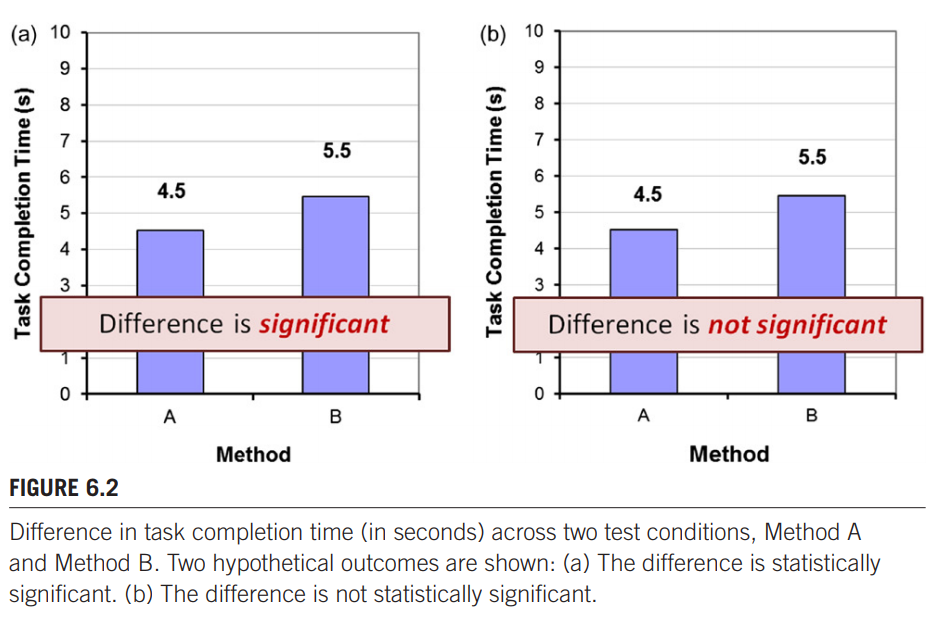
\includegraphics[width=0.8\linewidth]{result}
		\caption{Source: Fg. 6.2 (Mackenzie)}
	\end{figure}
	
\end{frame}

\begin{frame}
	\frametitle{Example: One-way with 2 levels} 
	\begin{figure}
		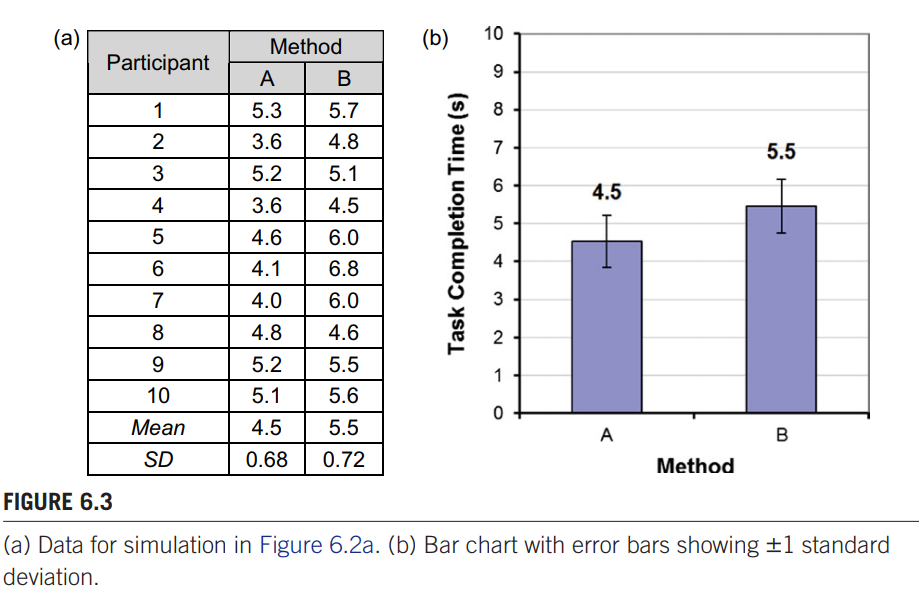
\includegraphics[width=0.8\linewidth]{resulta}
		\caption{Source: Fg. 6.3 (Mackenzie)}
	\end{figure}
	
\end{frame}

\begin{frame}
	\frametitle{Example: One-way with 2 levels with sig} 
	\begin{figure}
		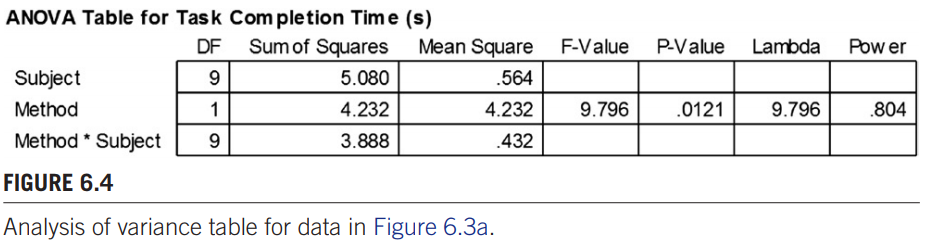
\includegraphics[width=0.6\linewidth]{resulta2}
		\caption{Source: Fg. 6.4 (Mackenzie): P-value of 0.0121 means that there is less than 2\% that the difference occurs by chance. By convention requires less than 0.05 to reject null hypothesis}
	\end{figure}
		\begin{figure}
		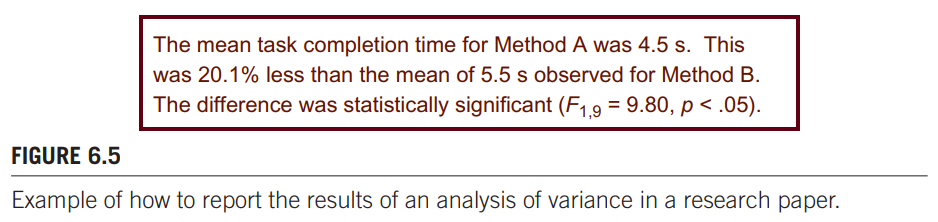
\includegraphics[width=0.8\linewidth]{resulta3}
		\caption{Source: Fg. 6.5 (Mackenzie): F-value is calculated = between-group variances / within-group variances = 4.232 / .432 }
	\end{figure}
\end{frame}

\begin{frame}
	\frametitle{Example: One-way with 2 levels with sig} 
	Reporting format (APA):
	\begin{itemize}
		\item If \textbf{significant}, use threshold set {.05, .01, .005, .001, .0005, .0001}.  \textit{p} is cited as \textit{p} $<$ .05 instead of \textit{p} $=$ .0121.   
		\item If \textbf{not significant though},  say "n.s." instead
		\item If \textbf{very close to significant}, report exact value.
		\item Plot with \textbf{standard error bars}
		\item Report \textbf{mean} and \textbf{std}  (same unit)
		\item Common nowadays to report\textbf{ effect size}
		\begin{itemize}
			\item  \textbf{Effect size}  measures how "strong" is the significance.  SPSS reports \textbf{Partial Eta Squared} ($\eta_{p}^{2}$) - .02 means that the factor X by itself accounted for only 2\% of the overall (effect + error) variance.  Usually around $>0.09$ is considered moderate, while $>0.25$ is large.
		\end{itemize}
	%		\item Must \textbf{strictly} follow the exact format for reporting - use parentheses, uppercase for \textit{F}, lowercase for \textit{p}, italics for \textit{F} and \textit{p}, space on both sides of equal sign, space after comma, space on both sides of the less than sign, degrees of freedom are subscript, three/four significant digits for \textit{F} statistics, does not require 0 in front of \textit{p}-value.
	\end{itemize}
\end{frame}

\begin{frame}
	\frametitle{Wide format}
	Since we are doing a \textbf{within-subject }design, this is also sometimes called \textbf{Repeated Measures ANOVA.}   In RP ANOVA,  it uses \textbf{wide format} data structure.
	\begin{figure}
		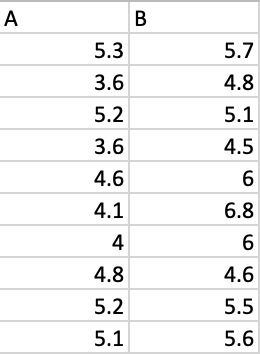
\includegraphics[width=0.2\linewidth]{wide-format}
		\caption{Wide format structure:  Cols depicting possible combinations}
	\end{figure}
\end{frame}

\begin{frame}
	\frametitle{Long format}
	Between-subject ANOVA (or ANOVA) uses \textbf{long format}.
	\begin{figure}
		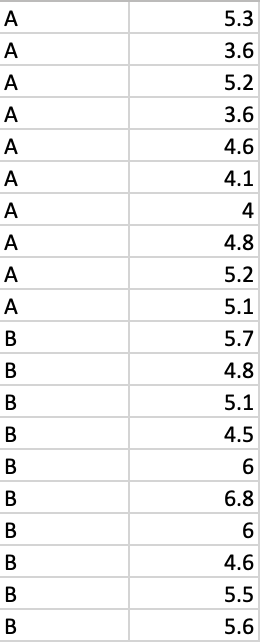
\includegraphics[width=0.2\linewidth]{long-format}
		\caption{Long format structure:  one col for each factor}
	\end{figure}
\end{frame}

\begin{frame}
	\frametitle{Example: One-way with 2 levels with no sig} 
	\begin{figure}
		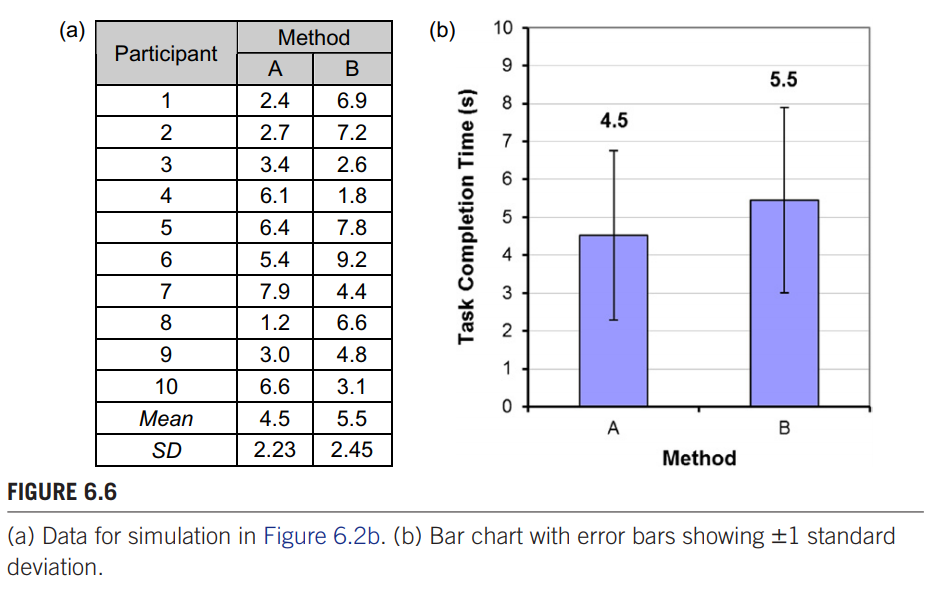
\includegraphics[width=0.8\linewidth]{resultb}
		\caption{Source: Fg. 6.6 (Mackenzie)}
	\end{figure}
\end{frame}
%
\begin{frame}
	\frametitle{Example: One-way with 2 levels with no sig} 
	\begin{figure}
		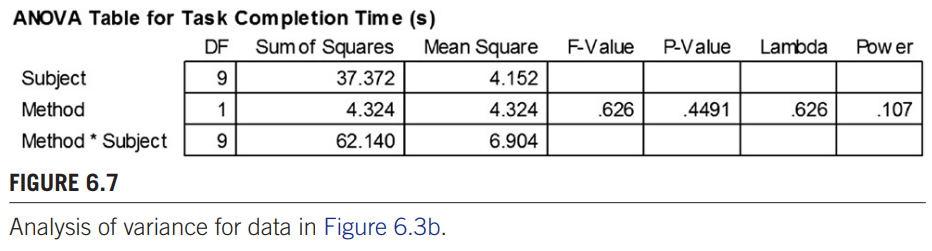
\includegraphics[width=0.55\linewidth]{resultb2}
		\caption{Source: Fg. 6.7 (Mackenzie). \textit{F} $=$ 4.324/6.904 = .626.  Given \textit{p}-value of .4491, there is around 45\% that the difference occurs by chance.}
	\end{figure}
	\begin{figure}
		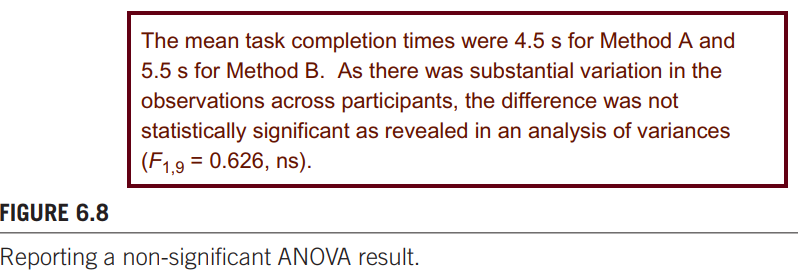
\includegraphics[width=0.55\linewidth]{resultb3}
		\caption{Source: Fg. 6.8 (Mackenzie).  It means that we have not enough evidence to reject null hypothesis, but it \textbf{does not mean that null hypothesis is true either}.}
	\end{figure}
\end{frame}

%\begin{frame}
%%	\footnotesize
%	\frametitle{Effect Size}
%%	Statistical considerations: 
%	\begin{itemize}
%%		\item \textbf{Type 1} error: false positive (say difference when there isn't); \textbf{Type II} error: false negative (say no difference when there is)
%%		\item To fix Type I error, we check \textit{p} value against our predefined significance level; this significance level is also called \textbf{alpha} (commonly .05 or less)
%		\item P-value only tell us significance, but not \textbf{strength}
%		
%%		\item \textbf{Power analysis} can be used prior to the experiment, to determine the sample size needed.  You need effect size, significance level(.05) and power (.7).  Note that this effect size could be eta-square, Cohen's d, or omega-squared depending on the tools you use.
%	\end{itemize}
%\end{frame}

%\begin{frame}
%%	\footnotesize
%	\frametitle{Effect Size}
%%	Statistical considerations: 
%	\begin{itemize}
%		\item The most common metrics are \textbf{eta squared} and \textbf{partial eta squared}.  The eta squared is a correlation ratio of SS-effect / SS-total, where SS-effect is sum of squares for the factor while SS-total is the total sum of square
%		\item However, when you have many IVs, eta-squared becomes too small.  To address this, we use partial eta-squared which is a ratio of SS-effect / (SS-effect+SS-error).  Here SS-error means the sum of squre for the error term.  
%		\item For eta-squared, 0.01 is small, 0.06 is medium, and 0.14 is large
%		\item For partial eta-squared, 0.01 (small), 0.09 (medium), and 0.25 (large)
%		\item Normally, eta-squared is fine for HCI experiment with around 2 to 3 IVs
%	\end{itemize}
%\end{frame}

\subsection{One-way with 4 levels}

\begin{frame}
	\frametitle{Example: One-way with 4 levels} 
	\begin{figure}
		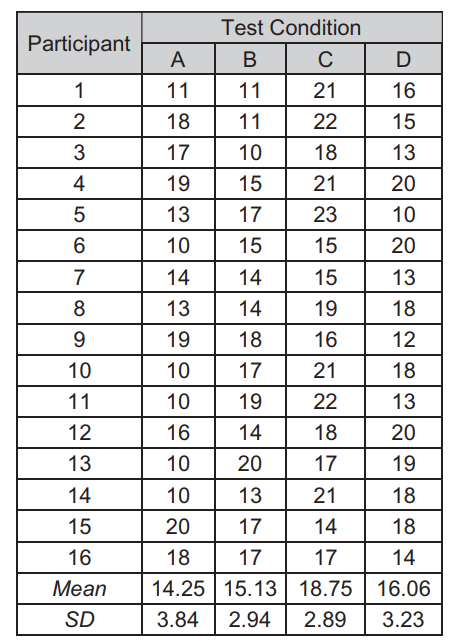
\includegraphics[width=0.35\linewidth]{4result}
		\caption{Source: Fg. 6.9a (Mackenzie)}
	\end{figure}
\end{frame}

\begin{frame}
	\frametitle{Example: One-way with 4 levels} 
	\begin{figure}
		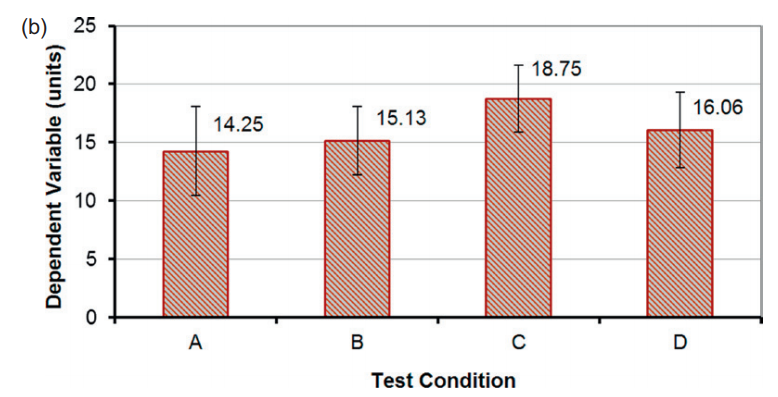
\includegraphics[width=0.6\linewidth]{4resulta}
		\caption{Source: Fg. 6.9b (Mackenzie)}
	\end{figure}
	\begin{figure}
	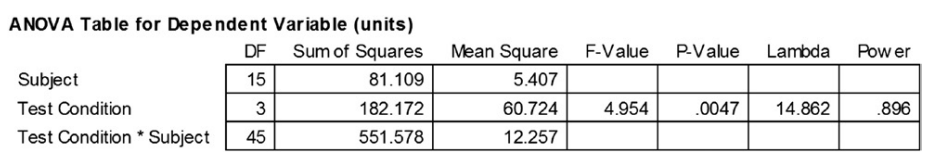
\includegraphics[width=0.8\linewidth]{4resultc}
	\caption{Source: Fg. 6.9c (Mackenzie)}
\end{figure}
\end{frame}

\begin{frame}
	\frametitle{Example: One-way with 4 levels} 
	\textbf{After ANOVA}, to determine exactly which condition is different with which condition, a \textbf{posthoc analysis} is required - either \textbf{Tukey's test} or \textbf{pairwise comparison with the Bonferroni correction}
	\begin{figure}
		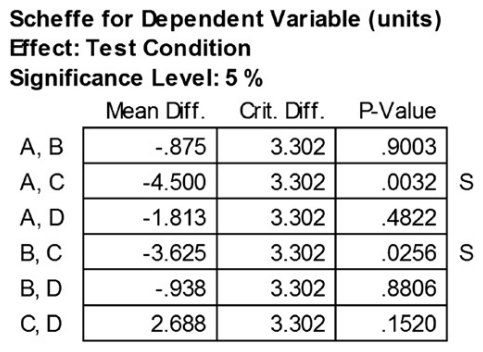
\includegraphics[width=0.5\linewidth]{posthoc}
		\caption{Source: Fg. 6.11 (Mackenzie)}
	\end{figure}
\end{frame}

\subsection{Between-subjects}

\begin{frame}
	\footnotesize
	\frametitle{Example: Between-subjects designs} 
	To check whether handedness has a effect on task completion time.
	\begin{figure}
		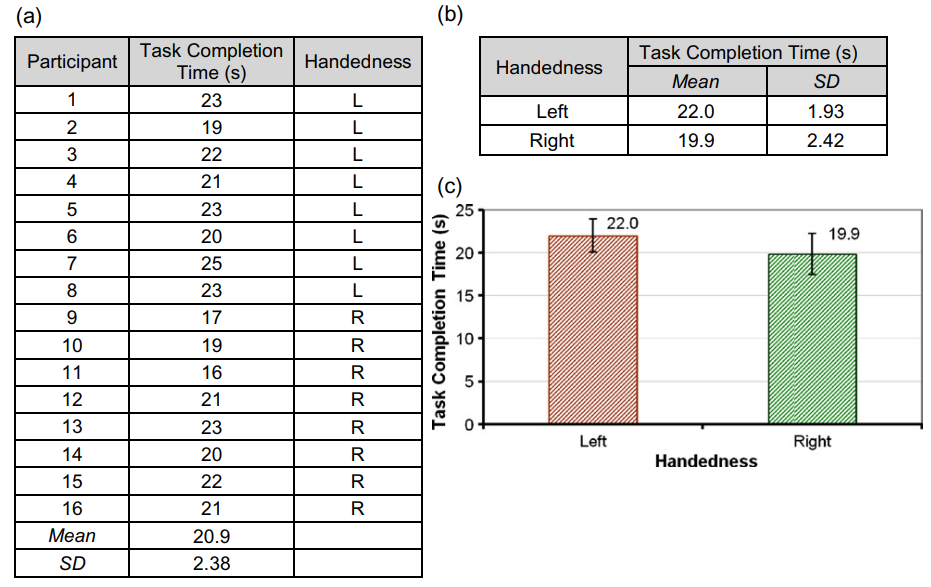
\includegraphics[width=0.5\linewidth]{between}
		\caption{Source: Fg. 6.12 (Mackenzie)}
	\end{figure}
	\begin{figure}
		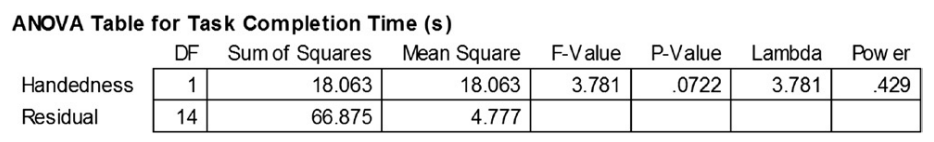
\includegraphics[width=0.6\linewidth]{between2}
		\caption{Source: Fg. 6.13 (Mackenzie)}
	\end{figure}
\end{frame}

\subsection{Two-way}

\begin{frame}
	\frametitle{Two-way ANOVA} 
	\begin{itemize}
		\item Experiments with two IVs (factors) is called a \textbf{two-way design}
		\item Analysis of variance of two-way design will give us \textbf{main effects} of each factor and \textbf{interaction effect}
		\item Interaction effect indicates a \textbf{relational effect} between the IV on the DV
%		\item If experiment has two factors, three possibilities are possible: 2 factors are both within-subject, or both are between-subject, or one is within and another is between.
	\end{itemize}
\end{frame}

\begin{frame}
	\frametitle{Interaction effects} 
		\begin{figure}
		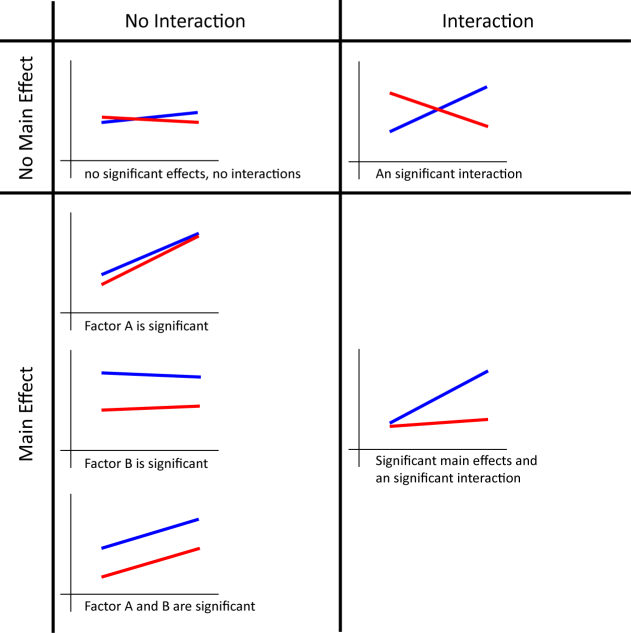
\includegraphics[width=0.5\linewidth]{interactions}
		\caption{Source: Yatani's post-hoc tests}
	\end{figure}
\end{frame}

\begin{frame}
	\footnotesize
	\frametitle{Example: 3 x 2 within-subjects design} 
	Let's take both factors as within-subjects, the first factor is device with 3 levels - mouse, trackball, and stylus, and second factor is task with 2 levels - point-select and drag-select.  We called this a 3 x 2 within-subjects design.
	\begin{figure}
		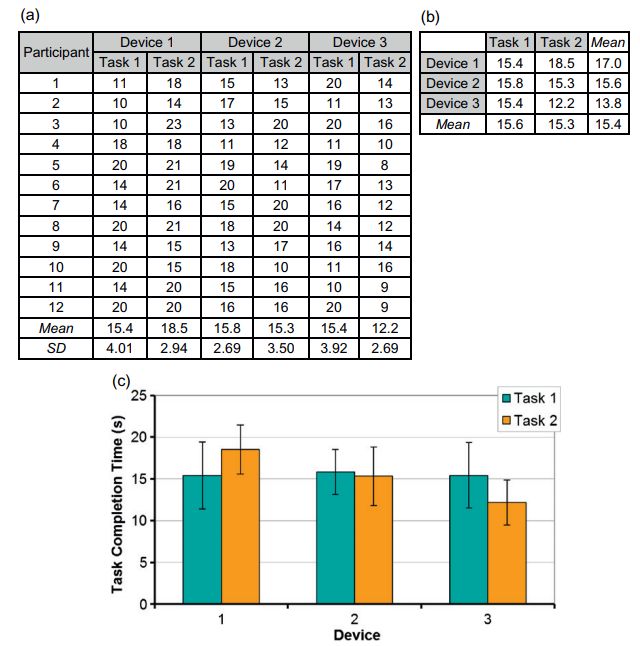
\includegraphics[width=0.43\linewidth]{2way}
		\caption{Source: Fg. 6.14 (Mackenzie)}
	\end{figure}
\end{frame}

\begin{frame}
	\footnotesize
	\frametitle{Example: 3 x 2 within-subjects design} 
	Three effects were observed - the main effect of device and task, and the interaction effect between device and task.
	\begin{figure}
		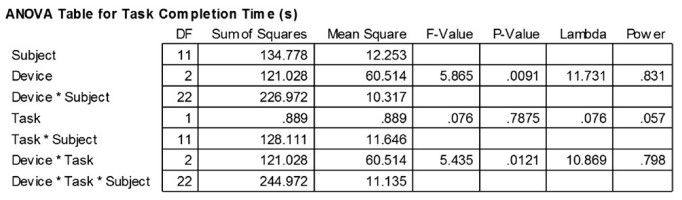
\includegraphics[width=0.9\linewidth]{2way-result}
		\caption{Source: Fg. 6.15 (Mackenzie)}
	\end{figure}
\end{frame}

\begin{frame}
	\frametitle{Example: 3 x 2 within-subjects design} 
	Reporting:
	\begin{figure}
		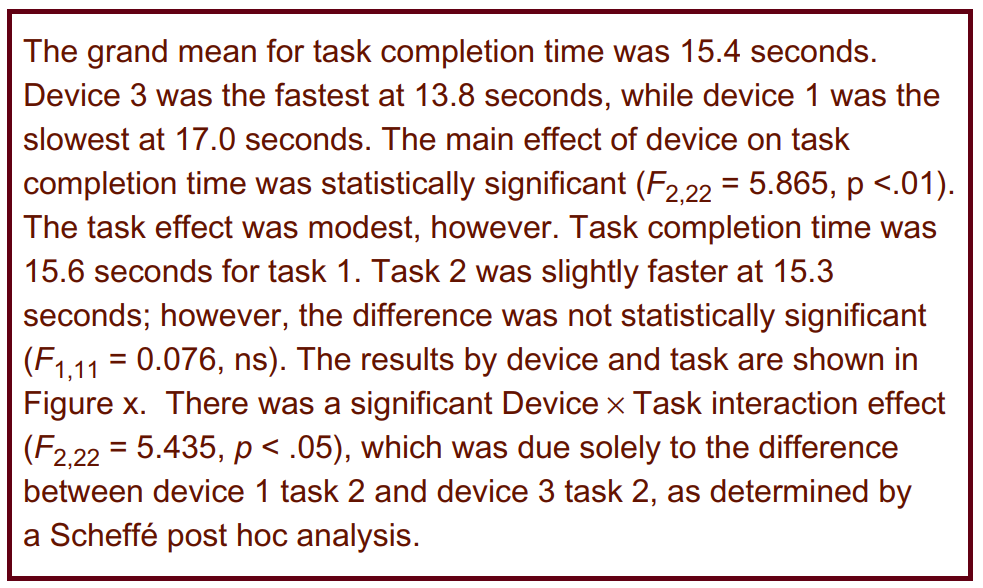
\includegraphics[width=0.7\linewidth]{2way-report}
		\caption{Source: Fg. 6.16 (Mackenzie)}
	\end{figure}
\end{frame}

%\subsection{Analysis of variance for counterbalancing testing}
%
%\begin{frame}
%	\frametitle{Analysis of variance for counterbalancing testing} 
%	\begin{itemize}
%		\item Let's say we counterbalance a single factor with two levels (A and B).  Group 1 (G1) does AB while Group 2 (G2) does BA.
%		\item How can we confirm that the counterbalancing works? We can use analysis of variance to check
%		\item We set a 2 x 2 mixed design with one within-subjects factor (method: A and B) and one between-subjects factor (groups: AB and BA)
%		\item If the ANOVA shows that group effect is not significant, it means our counterbalancing works.  
%		\item If there is an interaction effect between method and group, it represents a phenomenon known as \textbf{asymmetric skills transfer}, meaning that it was different transitioning from A to B than from B to A
%	\end{itemize}
%\end{frame}

%\begin{frame}
%\begin{center} 
%\usebeamerfont*{frametitle} \usebeamercolor[fg]{frametitle}  5-mins break 
%\end{center}
%\end{frame}

%------------------------------------------------
\section{Assumption check} % Sections can be created in order to organize your presentation into discrete blocks, all sections and subsections are automatically printed in the table of contents as an overview of the talk
%-----------------------------------------------

\begin{frame}
	\frametitle{Assumption check} 
%	\footnotesize
	\begin{itemize}
		\item To decide whether we can use ANOVA (also called parametric tests), we check the assumption of \textbf{normality} and \textbf{homogenity of variances}.  %Normally, if your data is \textbf{ratio}, it is safe to use parametric tests.  However, if unsure, one can also check for normality
	\end{itemize}
\end{frame}

\subsection{Normality check}

\begin{frame}
	\frametitle{Normality check} 
%	\footnotesize
	\begin{itemize}
		\item First easy way is to use \textbf{histogram} to check skewness
	\end{itemize}
	\begin{figure}
		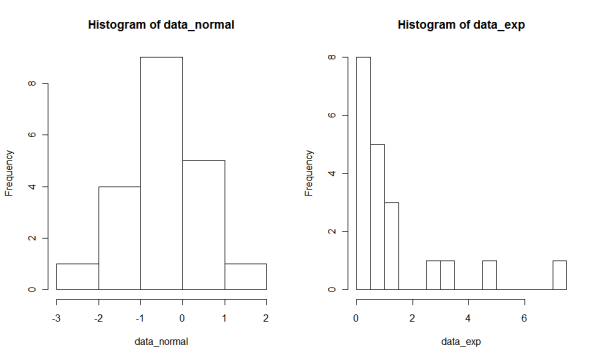
\includegraphics[width=0.8\linewidth]{histogram}
	\end{figure}
\end{frame}

\begin{frame}
	\frametitle{Normality check} 
%	\footnotesize
	\begin{itemize}
		\item Another way is to use \textbf{Q-Q plot}.  %It plots your data against an ideal normal distribution.  If the data points align approximately well with the line, it is normal.
	\end{itemize}
	\begin{figure}
		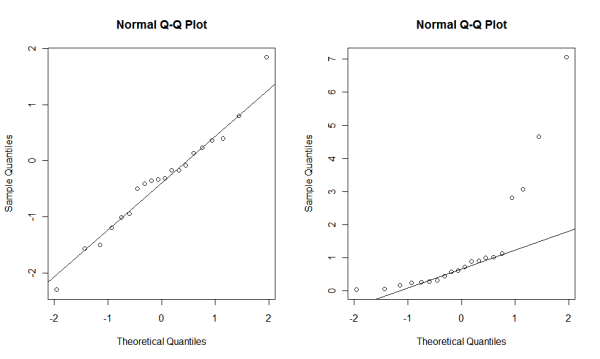
\includegraphics[width=0.8\linewidth]{qqplot}
	\end{figure}
\end{frame}

\begin{frame}
	\frametitle{Normality check} 
%	\footnotesize
	\begin{itemize}
		\item Two common tests for normality is \textbf{Shapiro Wilk} and \textbf{Kolmogorov-Smirnov} test %Another more mathematical way is statistical test which measures the difference of observed data against a known normal distribution.  
		\item Shapiro-Wilk is more appropriate for small sample sizes ($<$ 50)
%		\item Both of this test can be easily done in SPSS 
		\item For example, the null hypothesis of Shapiro-Wilk is that samples are taken from a normal distribution.  Here, \textbf{the p-value is larger than .05, thus is safe to say it's normal.}   The null hypothesis is same for Kolmogorov-Smirnov 
	\end{itemize}
	\begin{figure}
		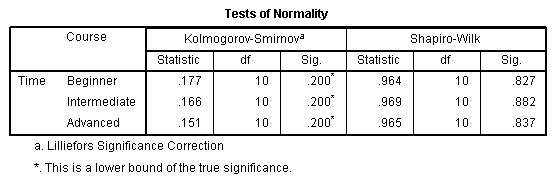
\includegraphics[width=0.8\linewidth]{normality}
	\end{figure}
\end{frame}

\subsection{Homogeneity of variances}

\begin{frame}
	\frametitle{Homogeneity of variances} 
%	\footnotesize
	\begin{itemize}
		\item t-test and ANOVA can handle differences in variances up to 4 times between smallest and largest (Howell, 2007)
		\item In a \textbf{between-subject }experiment, tests that can be use is \textbf{Levene's test} and \textbf{Bartlett's test} (p-value over 0.05 means that the variances are equal)
		\item In a\textbf{ repeated measures} experiment, \textbf{Sphericity test} is used instead (p-value over .05 means that sphericity has not been violated).   Note that in sphericity test, factors must have \textbf{more than 2 levels}.
	\end{itemize}
%	\begin{figure}
%		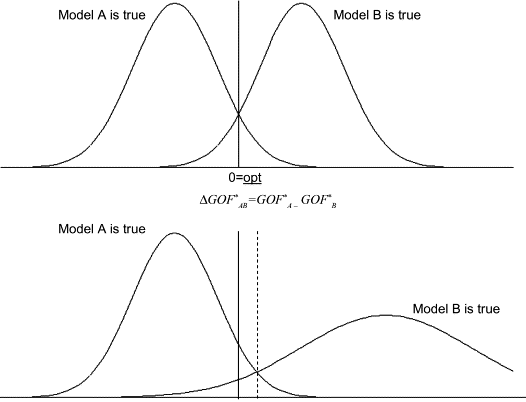
\includegraphics[width=0.5\linewidth]{homo}
%	\end{figure}
\end{frame}

%------------------------------------------------
%\section{Chi-square test} % Sections can be created in order to organize your presentation into discrete blocks, all sections and subsections are automatically printed in the table of contents as an overview of the talk
%%-----------------------------------------------
%
%\begin{frame}
%	\frametitle{Chi-square test} 
%	\begin{itemize}
%		\item Is a\textbf{ non-parametric tests} that is common for working with \textbf{counts/frequencies}
%		\item The test compares the observed values, against the expected values, which are developed under the assumption that there is no difference among groups.
%		\item Is non-parametric because it \textbf{does not work under any assumption of probability distribution}
%	\end{itemize}
%\end{frame}
%
%\begin{frame}
%	\frametitle{Example: Counts of usage} 
%	Consider how males and females scroll, either with mouse wheel (MW), clicking and dragging the scrollbar (CD), or keyboard (KB),
%	\begin{figure}
%		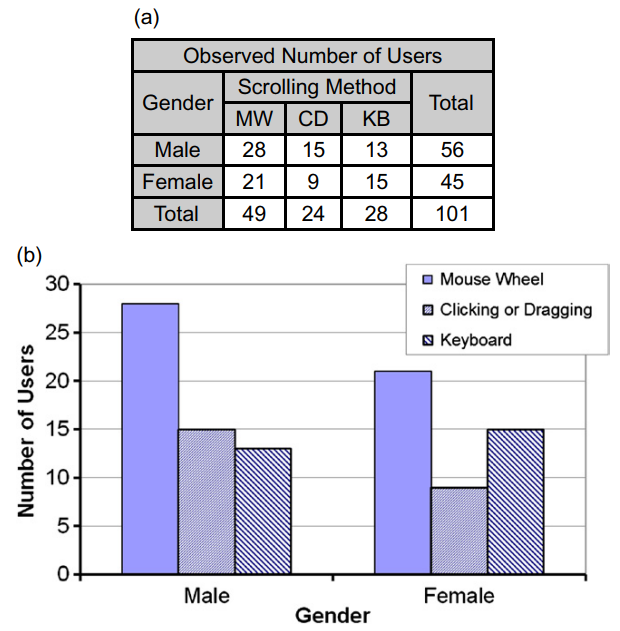
\includegraphics[width=0.45\linewidth]{chi}
%		\caption{Source: Fg. 6.22 (Mackenzie)}
%	\end{figure}
%\end{frame}
%
%\begin{frame}
%	\footnotesize
%	\frametitle{Example: Counts of usage} 
%	To determine the effect, the chi-square test is used.  The test statistics is written as ${\chi}^2$ using the lowercase Greek letter \textit{chi}.  Each expected value is the row total multiplied by the column total, divided by the grand total.  For example, Male-MW expected value is (56 x 49) /101 = 27.2.  Each chi square is simply the square of (observed - expected) / expected.  For example, Male-NW chi square is (28.0 - 27.2)$^2$/27.2 = 0.025
%	\begin{figure}
%		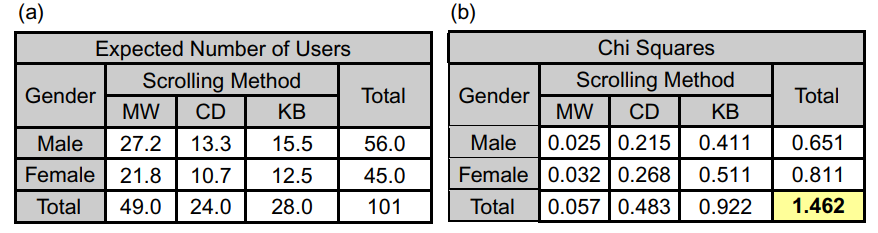
\includegraphics[width=0.9\linewidth]{chi-eg}
%		\caption{Source: Fg. 6.23 (Mackenzie)}
%	\end{figure}
%\end{frame}
%
%\begin{frame}
%	\footnotesize
%	\frametitle{Example: Counts of usage} 
%	Similar to F-statistic, we need to determine the critical value.  Given alpha of .05, and the degrees of freedom of (r-1)(c-1) = 2, we got the critical value as 5.99.  Since the observed value (1.462) is not larger than 5.99, there are no significant differences.  (\textit{Note that if there is a difference, a similar posthoc test can be subsequently performed to determine the differences between methods})
%	\begin{figure}
%		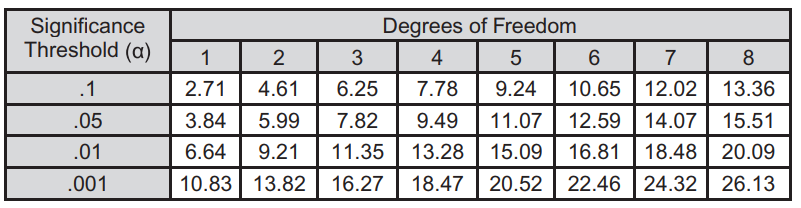
\includegraphics[width=0.9\linewidth]{chi-eg2}
%		\caption{Source: Fg. 6.24 (Mackenzie)}
%	\end{figure}
%\end{frame}

%------------------------------------------------
\section{Non-parametric tests} % Sections can be created in order to organize your presentation into discrete blocks, all sections and subsections are automatically printed in the table of contents as an overview of the talk
%-----------------------------------------------

\begin{frame}
	\frametitle{Non-parametric tests for ordinal data} 
	\begin{itemize}
		\item \textbf{Non-parametric test}s make no assumptions for probability distribution% thus are applicable to a wider range of data than parametric tests
		\item Downsides of non-parametric tests are \textbf{loss of information} %while parametric tests works on interval or ratio data, non-parametric tests deal with ordinal data (ranks)
%		\item Non-parametric tests ignore any property of the scale of data except ordinality
		\item For example, 49, 81, 82 are transformed to 1, 2, 3
		\item In HCI, non-parametric tests are often used for \textbf{questionnaires data} (e.g., using Likert scale) since they are \textbf{ordinal} data.  %Though non-parametric tests are limited to single factor analysis.
	\end{itemize}
\end{frame}

\begin{frame}
	\frametitle{Non-parametric tests for ordinal data} 
	Four most common non-parametric procedures that work based on the number of conditions and design %(\textit{Note that conditions here refer to \textbf{levels} of a single factor.  Also note that since Kruskal-Wallis aand Friedman operate or 3 or more conditions, a statistically significant outcome is usually followed with a post hoc pairwise comparisons})
	\begin{figure}
		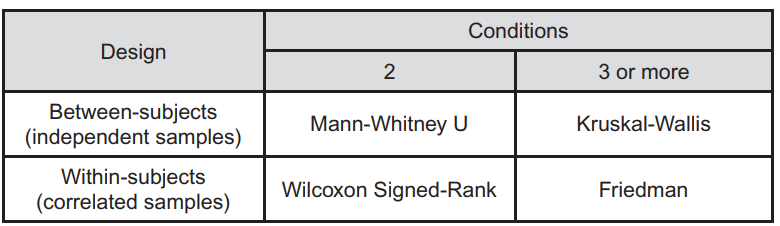
\includegraphics[width=0.9\linewidth]{6-29}
		\caption{Source: Fg. 6.29 (Mackenzie)}
	\end{figure}
\end{frame}

\begin{frame}
	\frametitle{Example: Mann-Whitney U} 
	10 Mac users and 10 PC users are interviewed about their political views on a 10-point linear scale (1 = very left, 2 = very right).  Turns out PC users are a little more "right-leaning"!
	\begin{figure}
		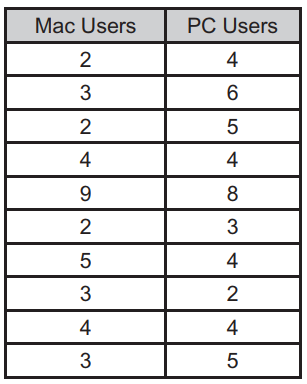
\includegraphics[width=0.3\linewidth]{6-30}
		\caption{Source: Fg. 6.30 (Mackenzie)}
	\end{figure}
\end{frame}


\begin{frame}
	\frametitle{Example:Mann-Whitney U} 
	\begin{itemize}
		\item Given 2 levels and between subject designs, \textbf{Mann-Whitney U} is suitable %Here, the data are potentially interval-scale but the intervals between successive codes are not equal, as the difference between 1 and 2 and 3 and 4 may not be equal (unlike temperature).  Since the data is at least ordinal, non-parametric tests are appropriate.  
		\item Here we found that \textit{p} = .1418, thus we conclude that no differences were found.
	\end{itemize}
	\begin{figure}
		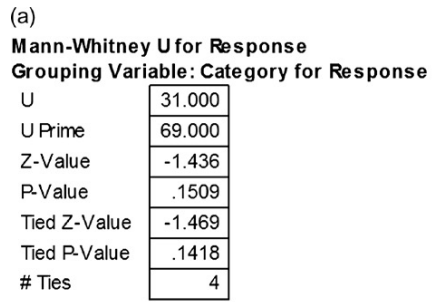
\includegraphics[width=0.4\linewidth]{6-31}
		\caption{Source: Fg. 6.31 (Mackenzie)}
	\end{figure}
\end{frame}

\begin{frame}
	\frametitle{Example: Wilcoxon Signed-Rank} 
	10 users rated the design of two media players on a 10-point linear scale (1 = not cool, 10 = really cool).  Which test should we use?
	\begin{figure}
		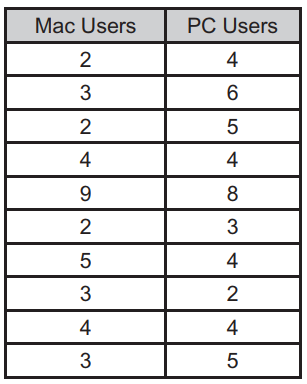
\includegraphics[width=0.3\linewidth]{6-30}
		\caption{Source: Fg. 6.32 (Mackenzie)}
	\end{figure}
\end{frame}

\begin{frame}
	\frametitle{Example: Wilcoxon Signed-Rank} 
	The Wilcoxon Signed-Rank test found that \textit{p} = .0242, thus we conclude that no differences were found.
	\begin{figure}
		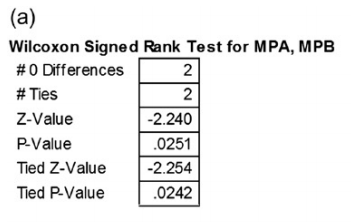
\includegraphics[width=0.6\linewidth]{6-33}
		\caption{Source: Fg. 6.33 (Mackenzie)}
	\end{figure}
\end{frame}

\begin{frame}
	\frametitle{Example: Kruskal-Wallis} 
	Is it significant?
	\begin{columns}[c] % The "c" option specifies centered vertical alignment while the "t" option is used for top vertical alignment
		
		\column{.5\textwidth} % Left column and width
		\begin{figure}
			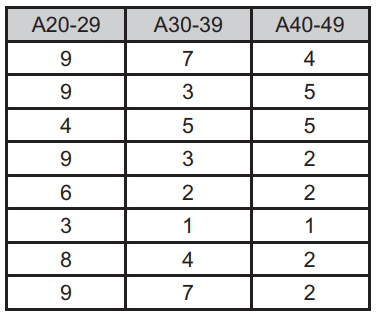
\includegraphics[width=0.8\linewidth]{6-34}
			\caption{Source: Fg. 6-34 (Mackenzie).}
		\end{figure}
		
		\column{.5\textwidth} % Right column and width
		\begin{figure}
			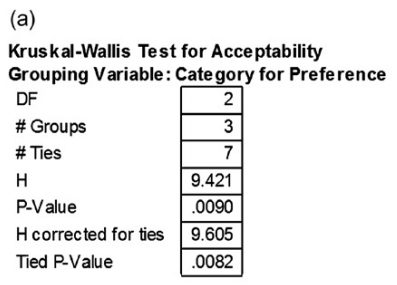
\includegraphics[width=0.9\linewidth]{6-35}
			\caption{Source: Fg. 6-35 (Mackenzie).}
		\end{figure}
	\end{columns}
\end{frame}

\begin{frame}
	\frametitle{Example: Kruskal-Wallis} 
	Since there are three conditions, we can further run post-hoc tests to find out the differences in pair.  Here, we found the difference between group 1 and 3.
	\begin{figure}
		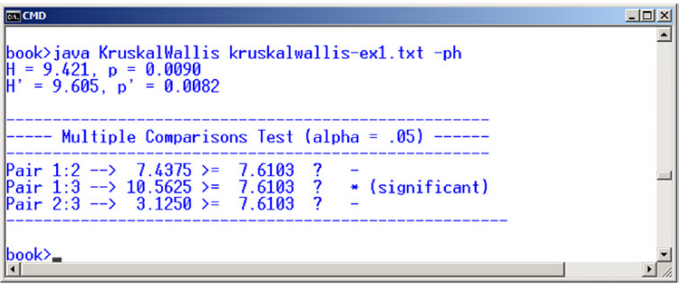
\includegraphics[width=0.6\linewidth]{6-36}
		\caption{Source: Fg. 6.36 (Mackenzie)}
	\end{figure}
\end{frame}

\begin{frame}
	\frametitle{Example: Friedman Test} 
 	So, what's the conclusion?
	\begin{columns}[c] % The "c" option specifies centered vertical alignment while the "t" option is used for top vertical alignment
		
		\column{.5\textwidth} % Left column and width
		\begin{figure}
			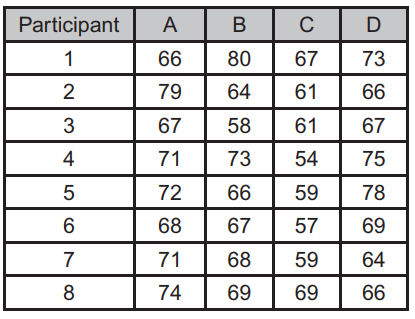
\includegraphics[width=0.65\linewidth]{6-37}
		\end{figure}
		
		\column{.5\textwidth} % Right column and width
		\begin{figure}
			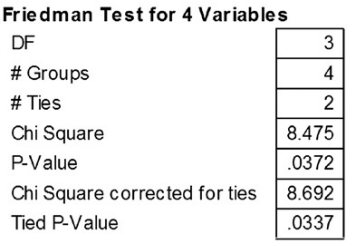
\includegraphics[width=0.75\linewidth]{6-38}
		\end{figure}
	\end{columns}
	\begin{figure}
		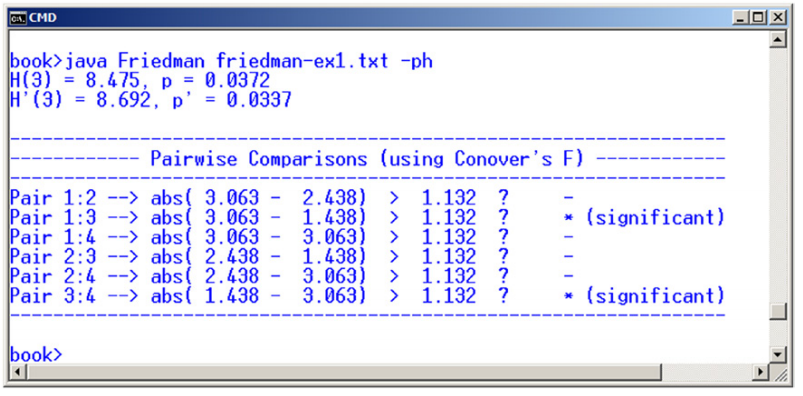
\includegraphics[width=0.4\linewidth]{6-39}
		\caption{Source: Fg. 6-(37-39) (Mackenzie).}
	\end{figure}
\end{frame}

%\begin{frame}
%	\frametitle{Statistical Procedures} 
%	\begin{itemize}
%		\item Statistical tests comes in two forms: \textbf{parametric} and \textbf{non-parametric test}
%		\item Parametric tests operate on data based on assumptions of a normal distribution or the t-distribution.
%		\item Non-parametric tests can operate on any data.
%		\item Parametric tests are superior to non-parametric tests, but require assumptions of distributions.
%	\end{itemize}
%	\begin{figure}
%	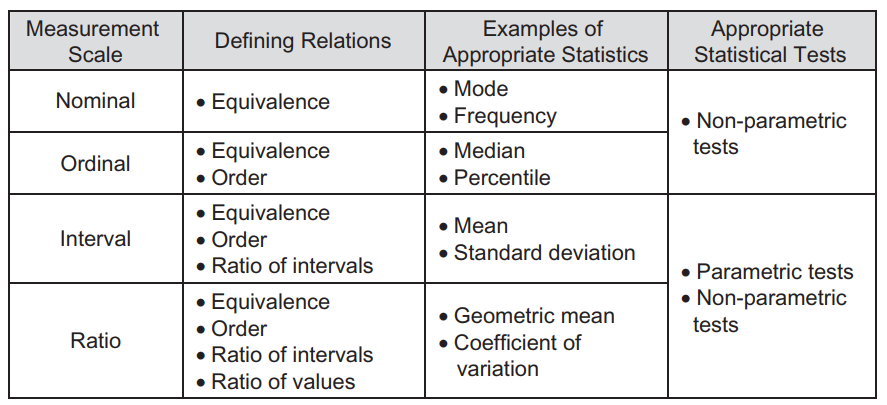
\includegraphics[width=0.6\linewidth]{stat}
%	\caption{Source: Fg. 6.1 (Mackenzie): Measurement scales of data, properties of data, and appropriate statistical tests}
%\end{figure}
%\end{frame}

%\begin{frame}
%	\frametitle{Assignment (Individual)}
%	Enjoy testing!  SPSS (free trial) is required.
%	\begin{figure}
%		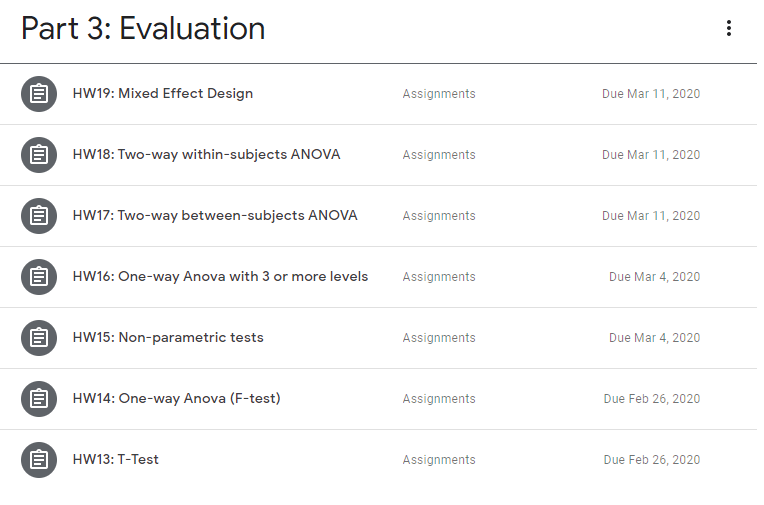
\includegraphics[width=0.9\linewidth]{assignment}
%	\end{figure}
%\end{frame}

%\begin{frame}
%	\frametitle{Reminders}
%	\begin{itemize}
%		\item Next week project proposal presentation.  Hard copy and soft copy as usual.
%		\item Next next week, please bring your pc, and install JASP.  We shall together do "Analysis of Variance" workshops for two weeks.
%	\end{itemize}
%\end{frame}

%\section{What's next}

\begin{frame}
\frametitle{What's next}
	\begin{itemize}
		\item Couple of workshops for ANOVA.  Please take a look at the \textbf{Tutorials} folder before coming to the class.   Make sure you have \textbf{JASP} installed.
		\item After we finish ANOVA, we gonna work on interaction and modeling,  download \textbf{GoFitts.jar} from the \textbf{Download} folder and make sure you can run it (you need Java).
	\end{itemize}
\end{frame}

\begin{frame}
\Huge{\centerline{Questions}}
\end{frame}

%----------------------------------------------------------------------------------------

\end{document} 